%This is a experiment example of ZhengXiaoyang's experiment report template

\documentclass[UTF8]{ctexart}
 
\usepackage{amsmath}
\usepackage{cases}
\usepackage{cite}
\usepackage{xeCJK}
\usepackage{graphicx}
\usepackage[margin=1in]{geometry}
\geometry{a4paper}
\usepackage{fancyhdr}
\pagestyle{fancy}
\fancyhf{}

\graphicspath{{picture/}}


\title{拉伸法测量杨氏模量}
\graphicspath{{picture/}}


\title{拉伸法测量杨氏模量预习报告}
\author{郑晓旸}
\date{\today}
\pagenumbering{arabic}

\begin{document}
%这里是文件的开头
\fancyhead[L]{郑晓旸}
\fancyhead[C]{杨氏模量}
\fancyfoot[C]{\thepage}

\maketitle
\tableofcontents
\newpage
\section{实验原理}

在弹性范围内,物体的形变量与外力成正比。描述这种关系的参数称为杨氏模量$E$,定义为
\begin{equation}
E=\frac{F/S}{\Delta L/L}=\frac{FL}{S\Delta L}
\end{equation}
其中$F$为外力,$S$为横截面积,$L$为原长,$\Delta L$为伸长量。

本实验采用光杠杆放大法测量金属丝的伸长量。如图\ref{fig:principle}所示,待测金属丝下端与光杠杆动足相连,上端固定。施加外力$F$后,金属丝伸长$\delta L$,带动光杠杆转过角度$\delta\theta$
\begin{equation}
\delta\theta\approx\frac{\delta L}{D}
\end{equation}
其中$D$为光杠杆动足到转轴的距离。反射镜偏转$\delta\theta$后,反射光线偏转$2\delta\theta$,在标尺上的位移为
\begin{equation}
\delta x\approx 2H\delta\theta=\frac{2H}{D}\delta L
\end{equation}
其中$H$为反射镜到标尺的距离。由此可知,光杠杆的放大倍数为$K=2H/D$。

\begin{figure}[htbp]
\centering
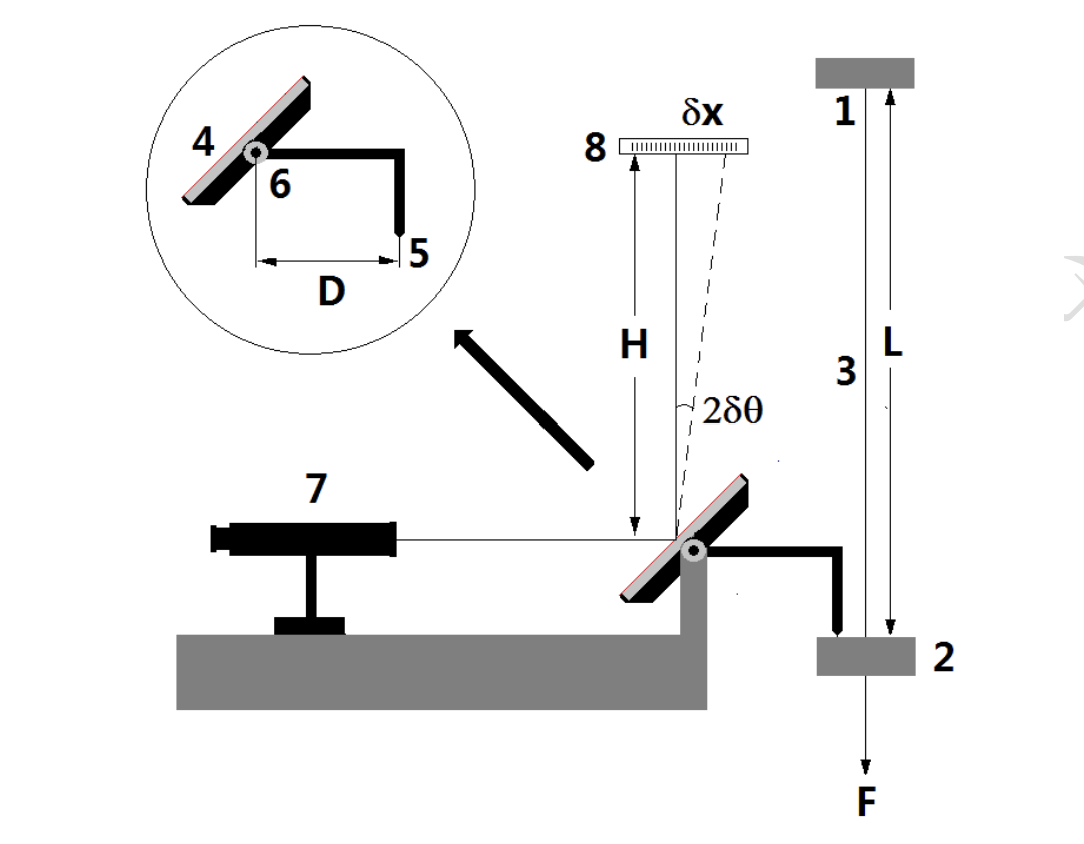
\includegraphics[width=0.6\textwidth]{principle.png}
\caption{光杠杆放大法原理图}
\label{fig:principle}
\end{figure}

将一系列外力$F_i$和对应的标尺读数$x_i$进行线性拟合
\begin{equation}
x_i=\alpha F_i+\beta
\end{equation}
然后根据斜率$\alpha$计算杨氏模量
\begin{equation}
E=\frac{8LH}{\pi d^2D\alpha}
\end{equation}
其中$d$为金属丝直径。

\section{实验过程}
\begin{enumerate}
    \item 调节测试架,连接信号线,打开数字拉力计,预热10min。
    \item 调节望远镜,使视野清晰,十字分划线与标尺刻度平行。
    \item 测量金属丝原长$L$、反射镜到标尺距离$H$、光杠杆常数$D$和金属丝直径$d$。
    \item 缓慢旋转施力螺母,每隔1kg记录一次标尺读数,测量加力和卸力两个过程。
    \item 数据处理,线性拟合$F_i-x_i$,计算杨氏模量$E$及其不确定度$u(E)$。
\end{enumerate}



\section{实验预习思考题}
\begin{enumerate}
    \item 推导光杠杆放大倍数公式。
    如图\ref{fig:principle}所示,金属丝伸长$\delta L$时,光杠杆转过角度
\begin{equation}
\delta\theta\approx\tan\delta\theta=\frac{\delta L}{D}
\end{equation}
反射光线偏转角度为$2\delta\theta$,在标尺上的位移
\begin{equation}
\delta x=H\tan(2\delta\theta)\approx 2H\delta\theta=\frac{2H}{D}\delta L
\end{equation}
所以光杠杆放大倍数为
\begin{equation}
K=\frac{\delta x}{\delta L}=\frac{2H}{D}
\end{equation}
    \item 为什么测量前要预先施加一些力?
    金属丝在自然状态下可能存在弯曲,直接测量会引入系统误差。预先施加一定的力,可以拉直金属丝,消除初始弯曲的影响。另外,这个预拉力应略大于测量力的下限,以保证测量过程中金属丝始终处于拉直状态。
    \item 实验中为什么要测量加力和减力两个过程的拉伸?
    测量材料在加卸载过程中的力学性能有两个目的:一是通过比较加卸载两条曲线的重合程度,判断测量是否在弹性变形范围内进行;二是取两条曲线的平均值,可以在一定程度上消除测试样品的滞弹性以及测试装置的机械迟滞等影响,提高测量精度。
    \item 证明杨氏模量不确定度的计算公式 \begin{equation} \frac{u(E)}{E}=\sqrt{(\frac{u(L)}{L})^2+(\frac{u(H)}{H})^2+(\frac{u(D)}{D})^2+(\frac{2u(d)}{d})^2+(\frac{u(\alpha)}{\alpha})^2} \end{equation}
    杨氏模量的计算公式为
    \begin{equation}
    E=\frac{8LH}{\pi d^2D\alpha}
    \end{equation}
    由不确定度传递公式,杨氏模量的相对不确定度
    \begin{equation}
    \frac{u(E)}{E}=\sqrt{(\frac{\partial\ln E}{\partial L}u(L))^2+(\frac{\partial\ln E}{\partial H}u(H))^2+(\frac{\partial\ln E}{\partial D}u(D))^2+(\frac{\partial\ln E}{\partial d}u(d))^2+(\frac{\partial\ln E}{\partial \alpha}u(\alpha))^2}
    \end{equation}
    其中
    \begin{equation}
    \frac{\partial\ln E}{\partial L}=\frac{1}{L},\ \frac{\partial\ln E}{\partial H}=\frac{1}{H},\ \frac{\partial\ln E}{\partial D}=-\frac{1}{D},\ \frac{\partial\ln E}{\partial d}=-\frac{2}{d},\ \frac{\partial\ln E}{\partial \alpha}=-\frac{1}{\alpha}
    \end{equation}
    代入可得
    \begin{equation}
    \frac{u(E)}{E}=\sqrt{(\frac{u(L)}{L})^2+(\frac{u(H)}{H})^2+(\frac{u(D)}{D})^2+(\frac{2u(d)}{d})^2+(\frac{u(\alpha)}{\alpha})^2}
    \end{equation}
    \item 如何计算(估算)$L,H,D,d,\alpha$的不确定度?
    对于单次测量的物理量$L,H,D,d$,其不确定度可按下式估算
    \begin{equation}
    u(x)=\frac{\Delta x}{\sqrt{3}}
    \end{equation}
    其中$\Delta x$为仪器的最小分度值。
    
    对于线性拟合得到的斜率$\alpha$,设拟合得到的直线方程为$y=\alpha x+\beta$,其斜率的不确定度为
    \begin{equation}
    u(\alpha)=\sqrt{\frac{\sum_{i=1}^n(y_i-\alpha x_i-\beta)^2}{(n-2)\sum_{i=1}^n(x_i-\bar{x})^2}}
    \end{equation}
    其中$\bar{x}$为$x_i$的平均值,$n$为数据点数。
\end{enumerate}





\end{document}
